\section*{Fundamentos}
La acetona ($C_3H_6 O $)  o también conocido como dimetil cetona, 2-propanona es un compuesto químico  muy versatil, se utiliza como materia prima para la producción de otros compuestos. La acetona tiene uso en un amplio campo de industrias. La Acetona se usa en la fabricación de plásticos, fibras y otros químicos además de usarse  como solvente \cite{quiroz2014diseno}. Asimismo, es muy usado como componente de cosméticos y como quita esmalte para las uñas. En la industria farmacéutica es muy usado como disolvente para la elaboración de distintos fármacos.

Como solvente, la acetona puede disolver muchos plásticos incluyendo botellas hechas de poliestireno, policarbonato y algunos tipos de polipropileno. Se caracteriza por ser uno de los disolventes orgánicos conocidos más usados, es  inmiscible en agua, además es fácilmente biodegradable llegando a ser encontrada en la naturaleza en plantas, árboles e incluso en el cuerpo humano debido a procesos de degradación de grasas \cite{garcia2020ingenieria}. En el laboratorio este químico es usado como disolvente aprótico polar en una gran variedad de reacciones orgánicas. En la industria minera es usada ampliamente para el transporte y almacenamiento seguro de acetileno, los tanques que contiene un material poroso primero son llenados con acetona y posteriormente con acetileno que se disuelve en la acetona \cite{abdullah2017production}. En la industria cosmética este producto es ampliamente usado y también está listado como componente en aditivos y envolturas alimenticias. Los dermatólogos la usan con alcohol en tratamientos de acné para desprender la piel muerta. También es usada como agente de secado debido a la facilidad con la que se mezcla en agua. Algo importante a considerar  es que la acetona tiende a crear azeotropos  con sustancias no polares como alifáticos. \\

\begin{multicols}{2}

    \subsection*{Reacción}

    La producción de Acetona tiene múltiples formas de obtenerse: Via cumeno, Oxidación de propeno,  deshidrigenación de IPA, Oxidación del diisopropilbenceno, Ácido Acético  y mediante acetileno

    Se puede obtener acetona mediante la deshidrogenación catalítica de alcohol isopropílico vaporizado, calentado e introducido en un reactor 250-270 $^{\circ} $ C \cite{acevedotrabajo}.
    La reacción se lleva a cabo mediante la siguiente ecuación:

            $$ (CH_3)_{2}CHOH  \rightarrow (CH_3)_2CO + H_2 $$

    Para la reacción de oxidación del Alcohol Isopropìlico se utiliza catalizadores metálicos de Cobre, aleaciones de Cobre y Plata; y óxidos metálicos de Cobre, aleaciones de Cobre y más fácil de regular que la deshidrogenación. La temperatura de la reacción varía en el rango de 200 y 800 \cite{quiroz2014diseno}.
    En la Figura \ref{fig:my_label} se presenta la secuencia del proceso en forma de un diagrama de bloques.

        \begin{figure}[H]
            \centering
            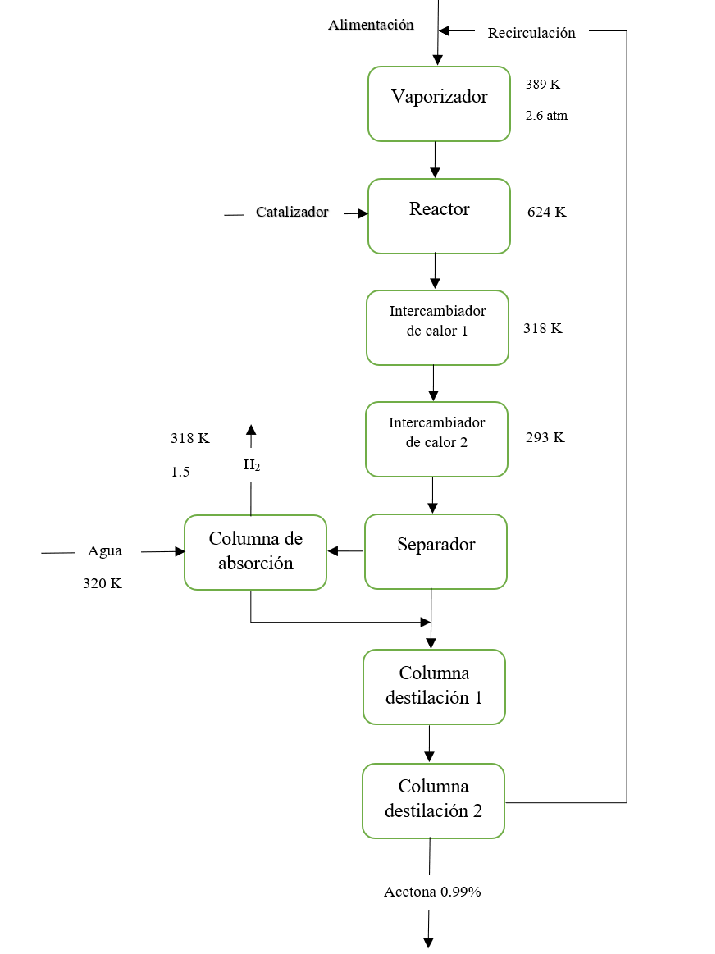
\includegraphics[scale=0.7]{images/Diagrama_completo.pdf}
            \caption{Diagrama de bloques del proceso}
            \label{fig:my_label}
        \end{figure}


\end{multicols}

    La principal ventaja de este proceso es que la acetona producida está libre de trazas de compuestos aromáticos, en particular benceno. Por esta razón la acetona producida a partir de alcohol isopropílico puede ser preferida por la industria farmacéutica, debido a las fuertes restricciones del uso de solventes.

    Al comienzo del proceso, la alimentación que contiene alcohol isopropílico y agua,  se mezcla con  la corriente de reciclaje  en el tambor de alimentación. Desde aquí, esta mezcla se envía al vaporizador, para cambiar la fase de la corriente como vapor. Después del vaporizador, la mezcla se calienta hasta la temperatura de reacción en el calentador.

    Acetona, hidrógeno gas $(H_2)$ se producen, y se descargan agua y alcohol isopropílico. La mezcla que son acetona, hidrógeno, agua y alcohol isopropílico se envían al enfriador y luego a un condensador. Después del condensador, la mezcla se envía al separador flash. Se obtiene hidrógeno, acetona, alcohol isopropílico y agua como producto superior. Este producto superior se envía a una torre de absorción para eliminar el hidrógeno. El producto inferior del separador flash que se compone de acetona, agua y alcohol isopropílico se mezclan con el producto de fondo de la columna de absorción antes de la primera columna de destilación. En esta, la acetona se obtiene del producto superior con 99\% en peso. La salida de la primera columna se envían a la segunda columna de destilación. Se envía el producto superior de la segunda columna para alimentar el tambor y el producto del fondo se desecha como agua residual \cite{article}.

    El la Figura \ref{fig:Diagrama} se muestra un diagrama  de proceso que muestra la ruta que sigue a través de los distintos equipos para la producción de acetona.
        \begin{figure}[H]
            \centering
            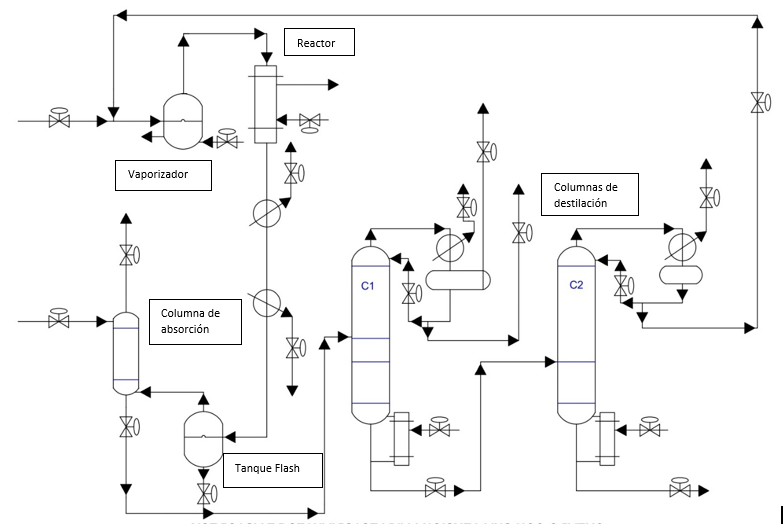
\includegraphics[scale = 0.55]{images/Diagrama_CAD.png}
            \caption{Diagrama del proceso.}
            \label{fig:Diagrama}
        \end{figure}

    \subsection*{Sistema de control}

    De las posibles opciones de control que existen dentro del sistema, se estudiaron las diversas posibilidades de los equipos de procesos y se toma la decisión de optar por la controlar la temperatura del reactor controlado la apertura de la válvula de  la chaqueta.
    \paragraph{}
    Para alcanzar los objetivos planteados en cuanto a obtener propuesta de control  es necesario tener en consideración el proceso dinámico del sistema. Para lograr el control automático de procesos se requiere del diseño e implementación de un
    sistema de control \cite{smith1991control}. Se debe considerar un objetivo de control. En este trabajo se plantea  como tal la temperatura del reactor . Se realizara mediante las ecuaciones descritas  anteriormente.
    La  reacción  del reactor  es:\\
                $$ A \rightarrow B +    C $$
    Donde $A$ es IPA, $B$ es la acetona  y $C$ es $H_2$\\
    Los balances de masa y energía  son:\\
        \begin{equation}
            \dfrac{dC_A}{dt}= r_A -\dfrac{F (C_{A0}-C_A)}{V}
            \label{balanceA}
        \end{equation}

        \begin{equation}
            \dfrac{dC_B}{dt}= -r_A +\dfrac{F(C_{B0}- C_B)}{V}
        \end{equation}

        \begin{equation}
            \dfrac{dC_C}{dt}= r_A +\dfrac{F(C_{C0} - C_C)}{V}
        \end{equation}

    Para el balance energía se tiene que:
        \begin{equation}
            \dfrac{dT_r}{dt} = \dfrac{F_r(T_f - T_r)}{V_r} + \dfrac{-\Delta H_{rxn}}{\rho_r C_{pr}}k_0exp\left(\frac{-E}{RT_r}\right)C_A -\dfrac{UA(T_r-T_j)}{V_r\rho_r C_{pr}}
            \label{energia}
        \end{equation}

        \begin{equation}
            \dfrac{dT_j}{dt} = \dfrac{F_j(T_{j0} - T_j)}{V_j}  +\dfrac{UA(T_r-T_j)}{V_j\rho_j C_{pj}}
            \label{energiachaqueta}
        \end{equation}

    Donde:

\begin{multicols}{2}
\paragraph{}

$C_A $ = Concentración de $A$\\
$C_B $ =Concentración de $B$\\
$C_C $ =Concentración de $C$\\
$C_{A0} $ =Concentración inicial de $A$\\
$C_{B0} $ =Concentración inicial de $B$\\
$C_{C0} $ =Concentración inicial de $C$\\
$U$ = Coeficiente global de transferencia de calor \\
$A$ = Área del intercambiador\\
$T_f$ = Temperatura de entrada\\
$T_j $ = Temperatura de la chaqueta\\
$F_r$ =  Flujo de entrada del reactor\\
$F_j$ =  Flujo de entrada  de la chaqueta\\
$ T_r $ =  Temperatura del reactor\\
$E $= Energía de activación\\
$R $= Constante de los gases ideales\\
$V_r $= Volumen de reactor\\
$V_j $= Volumen de la chaqueta\\
$ \rho_r $ = Densidad del flujo  de entrada al reactor\\
$ \rho_j $ = Densidad del flujo  de entrada a la chaqueta\\
$C_{pr}$= Capacidad calorífica del flujo de entrada al reactor\\
$C_{pj}$= Capacidad calorífica del flujo de entrada a la chaqueta\\
$ k_0$= Constante de reacción cinética \\
$\Delta H_{rxn}$ =  $\Delta H$ de reacción

\end{multicols}
